\documentclass[12pt]{jsarticle}
\usepackage{fancyhdr}
\pagestyle{fancy}
\lhead{\leftmark}
\rhead{\today}

\usepackage{graphicx}

\begin{document}

\title{
  ギガマシーンダービィ \linebreak{}
  エナドリ爆発 (仮) \linebreak{}
  企画書/仕様書
}
\author{nasuria}
\date{\today}
\maketitle
\newpage

\tableofcontents
\newpage


\section{概要}
大学生がエナドリを投げて敵を倒し、ステージを進む2Dアクション。

主人公の攻撃はチャージで形態が変わり、だんだん強化される。

\begin{figure}[htbp]
  \begin{center}
    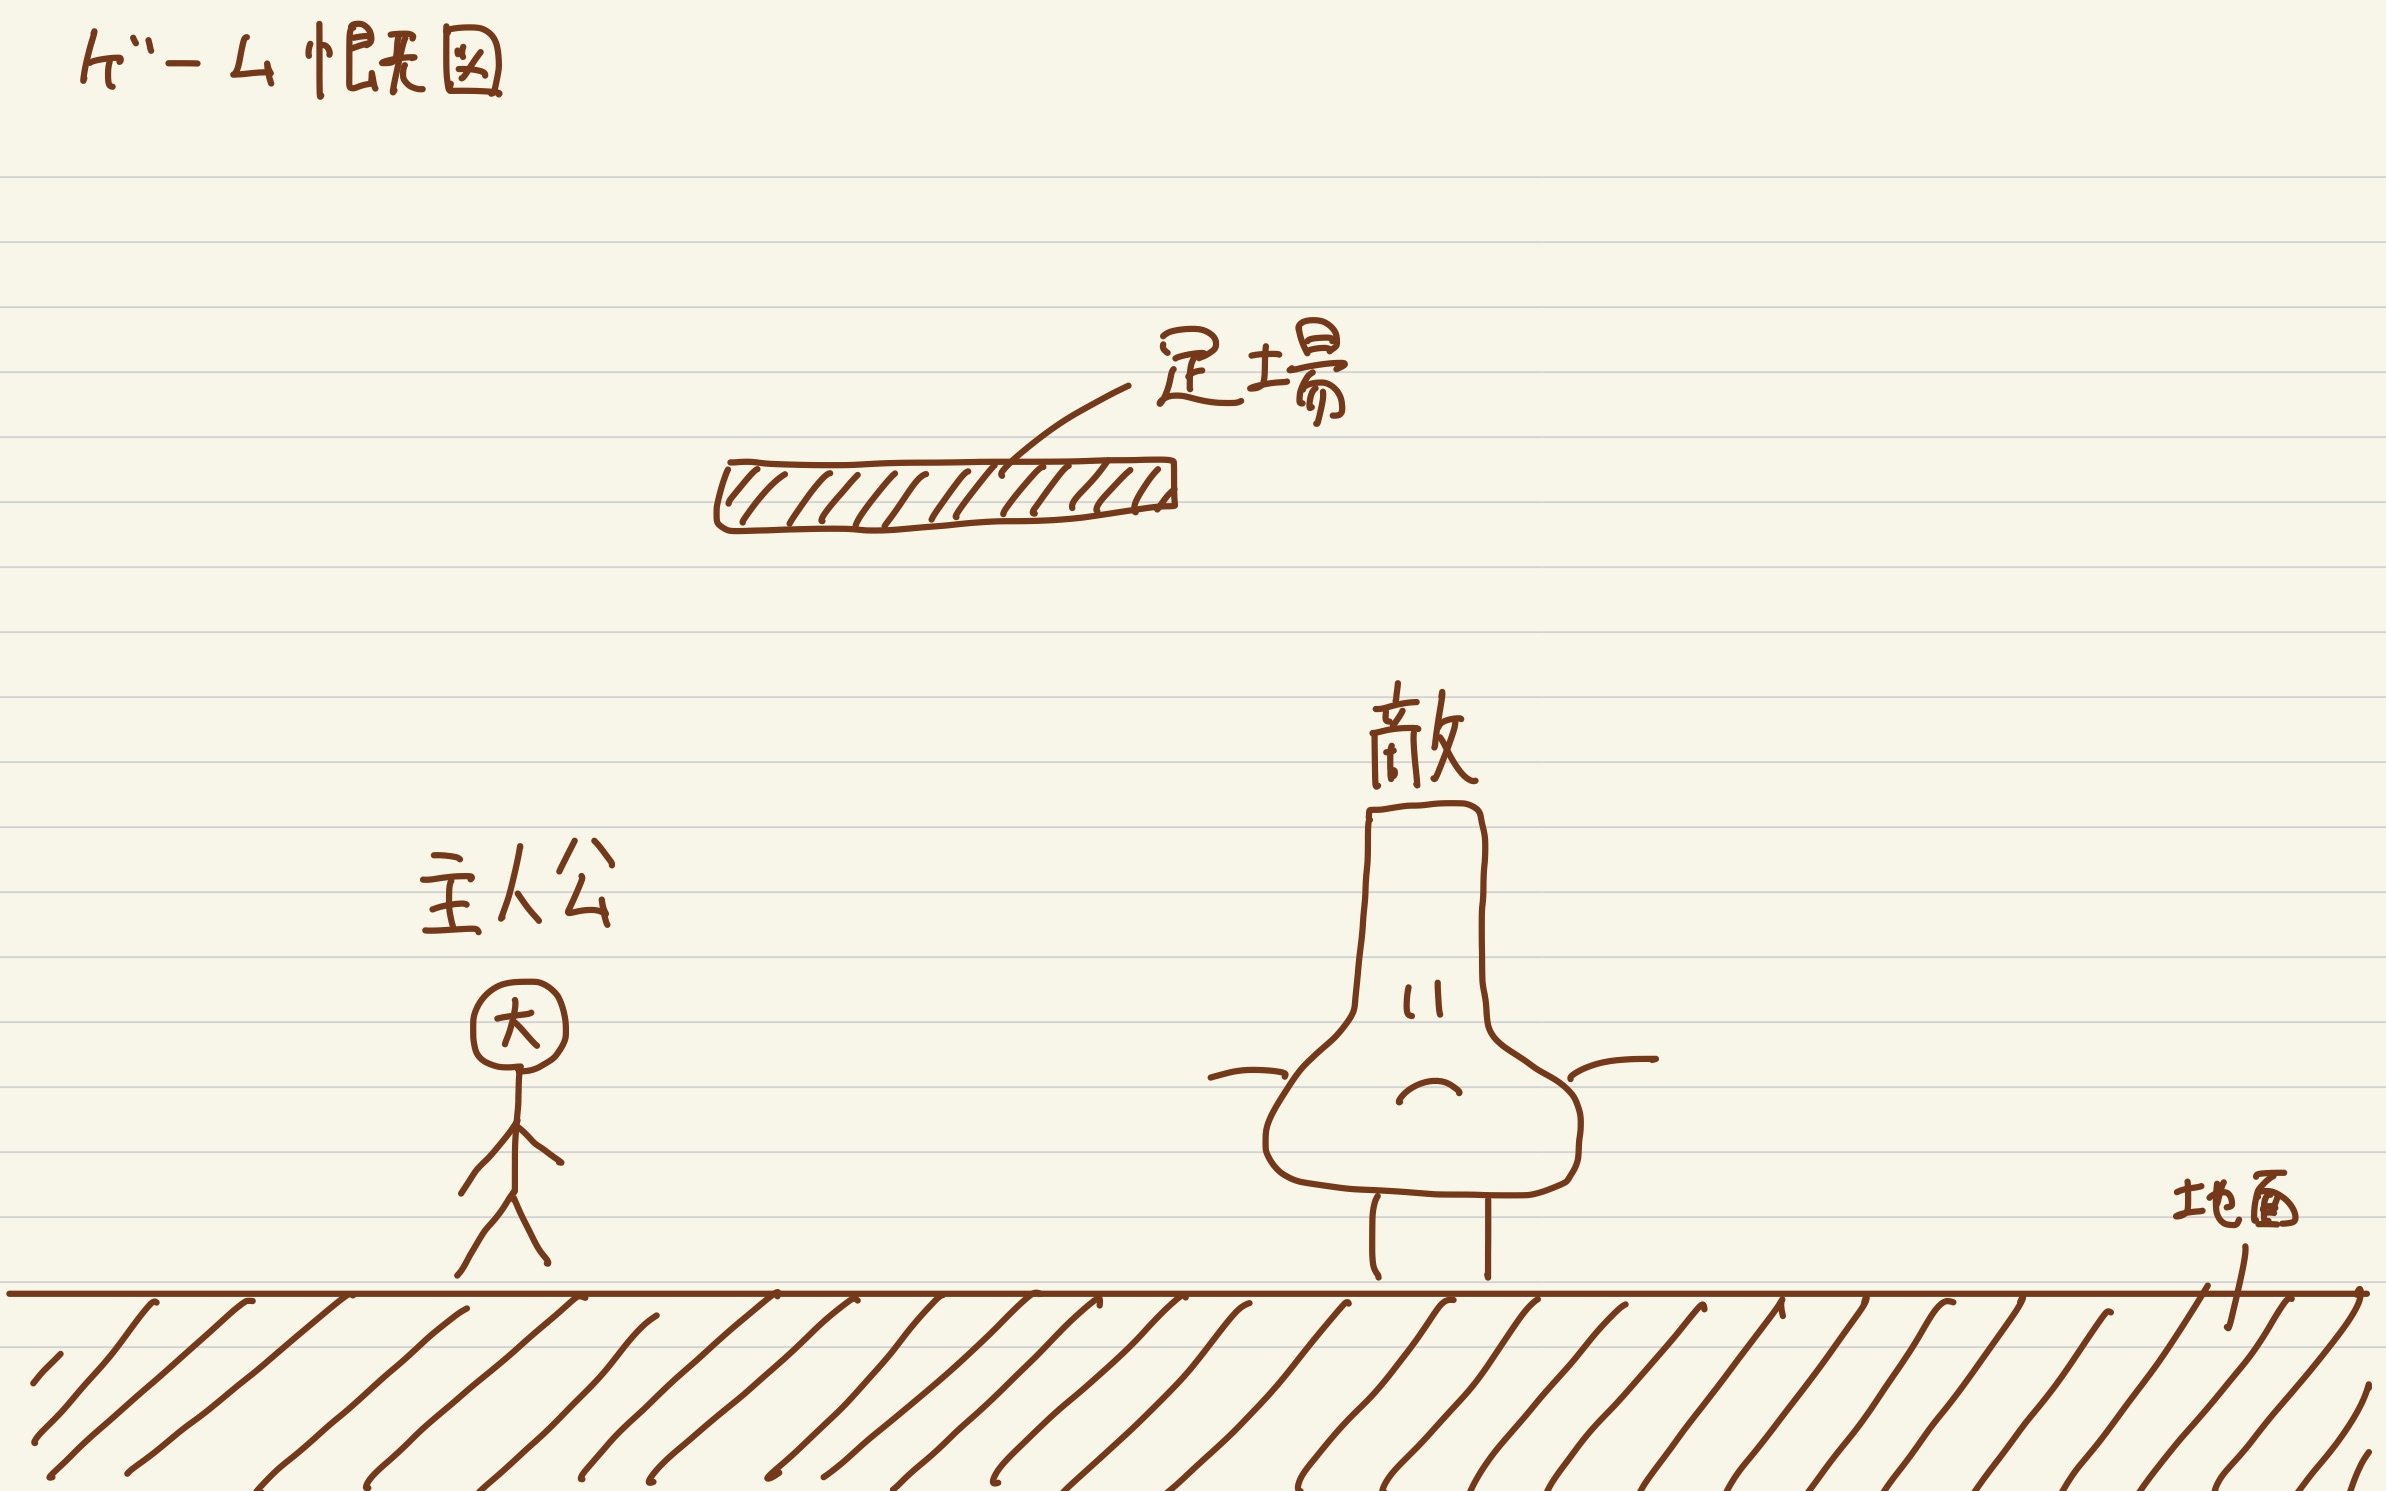
\includegraphics[width=12cm]{imags/gameGaizu.eps}
    \caption{ゲーム概図}
  \end{center}
\end{figure}

\newpage

\section{主人公-大学生}
\subsection{アクション}
\subsubsection{左右移動}

大学生が右左に動く。

\begin{figure}[htbp]
  \begin{center}
    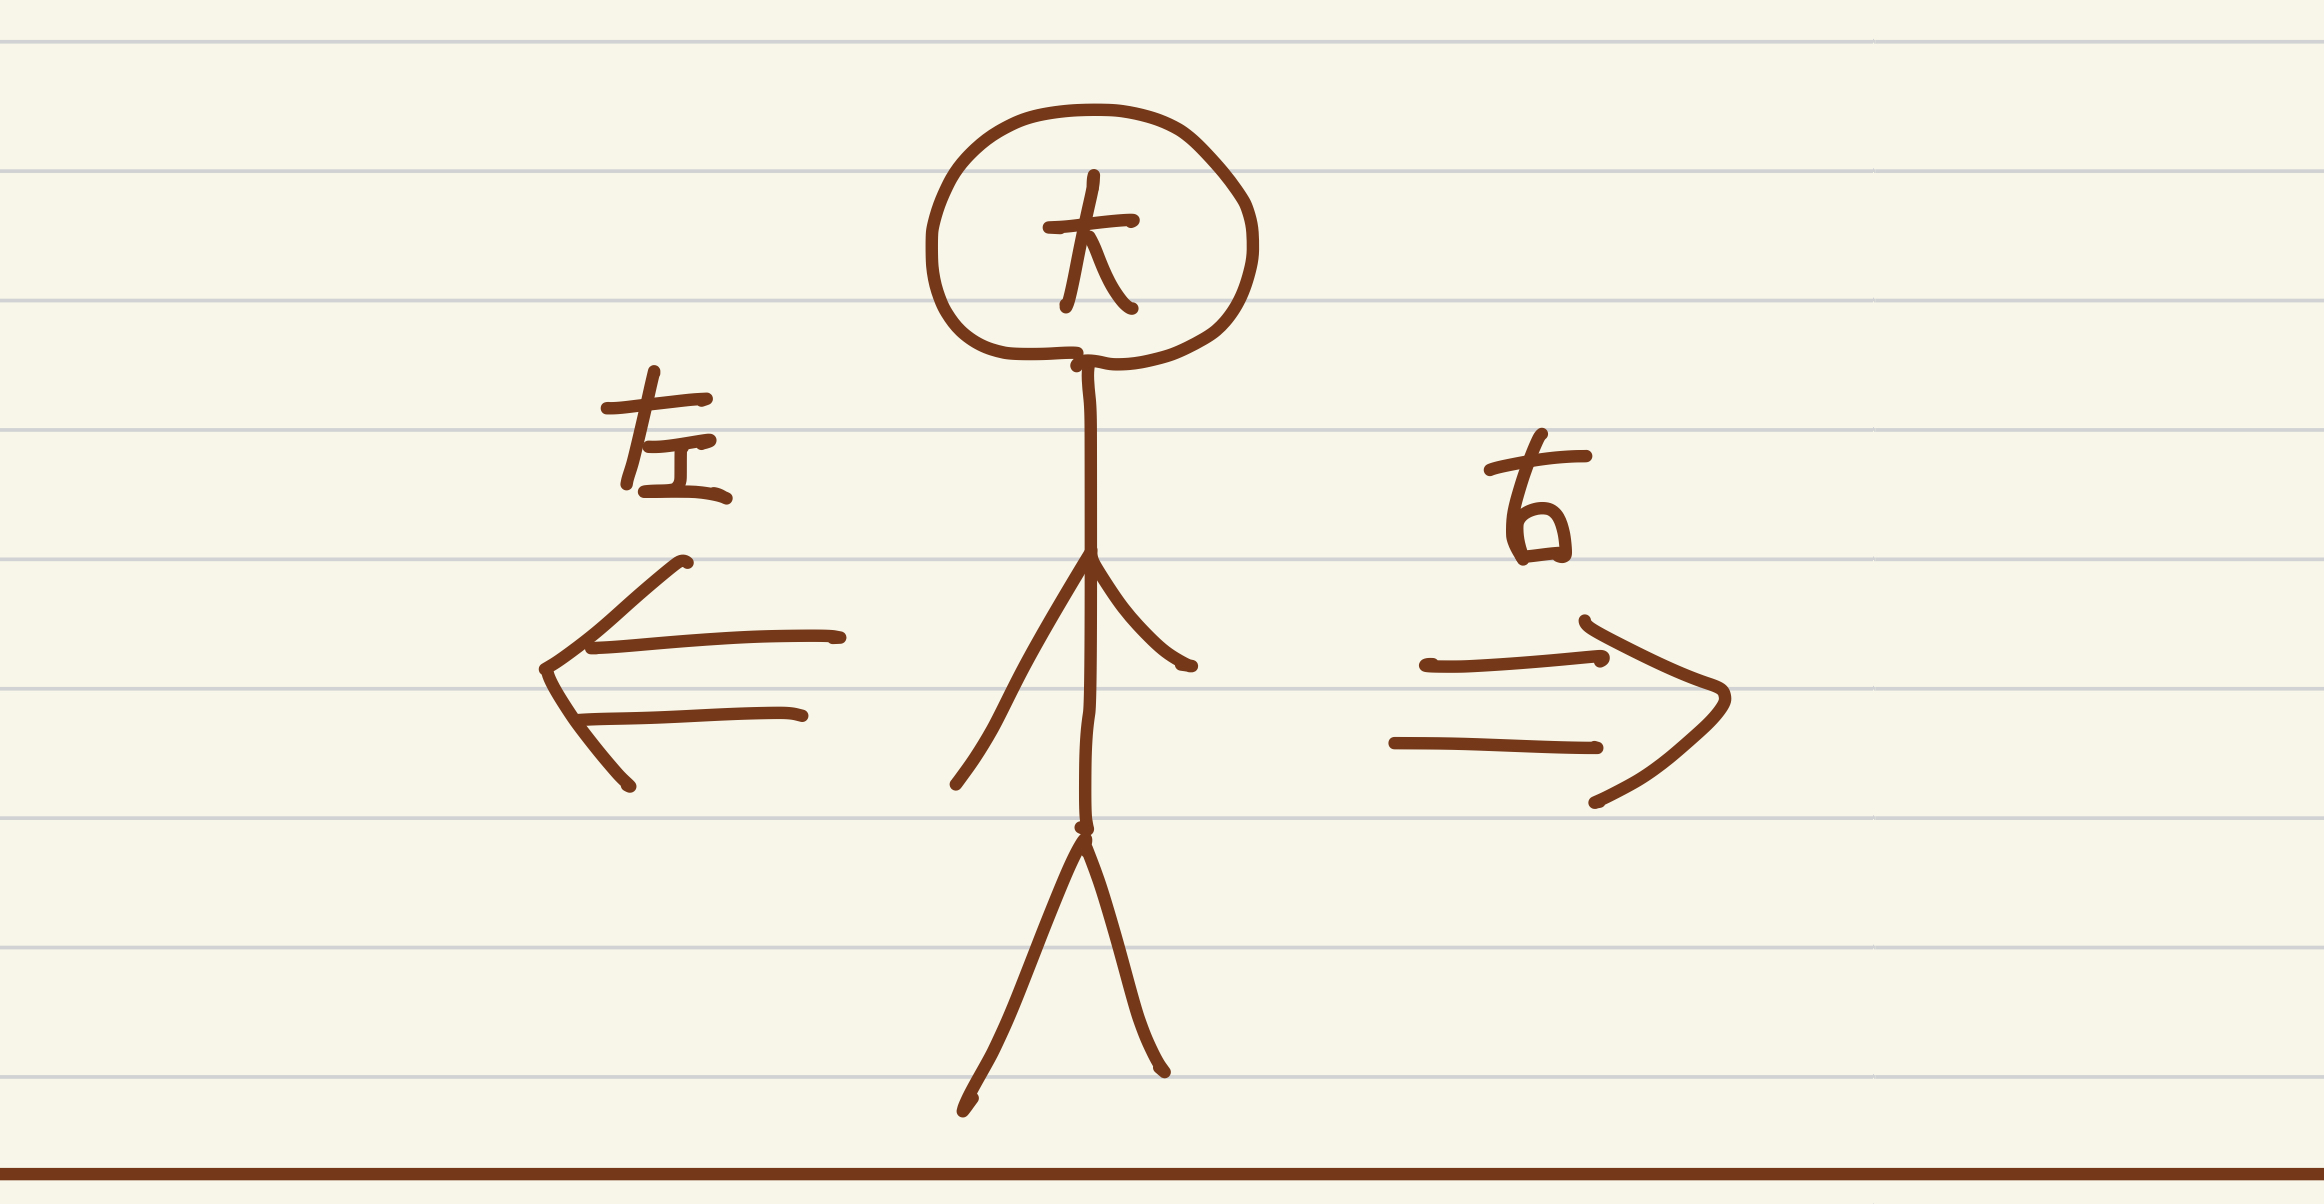
\includegraphics[width=8cm]{imags/daigakuseiSayuu.eps}
    \caption{左右に動く大学生}
  \end{center}
\end{figure}

\begin{table}[htbp]
  \centering
  \caption{PCでの左右移動のキー対応}
  \begin{tabular}{c|c}
    動作 & 対応するキー \\
    \hline
    右に動く & 右矢印キー \\
      & Dキー \\
    \hline
    左に動く & 矢印左キー \\
      & Aキー \\
  \end{tabular}
\end{table}

\begin{table}[htbp]
  \centering
  \caption{コントローラーでの左右移動のボタン対応}
  \begin{tabular}{c|c}
    動作 & 対応するボタン\\
    \hline
    右に動く & 右方向ボタン \\
      & Lスティックを右に \\
    \hline
    左に動く & 左方向ボタン \\
      & Lスティックを左に
  \end{tabular}
\end{table}

\newpage

\begin{figure}[htbp]
  \begin{center}
    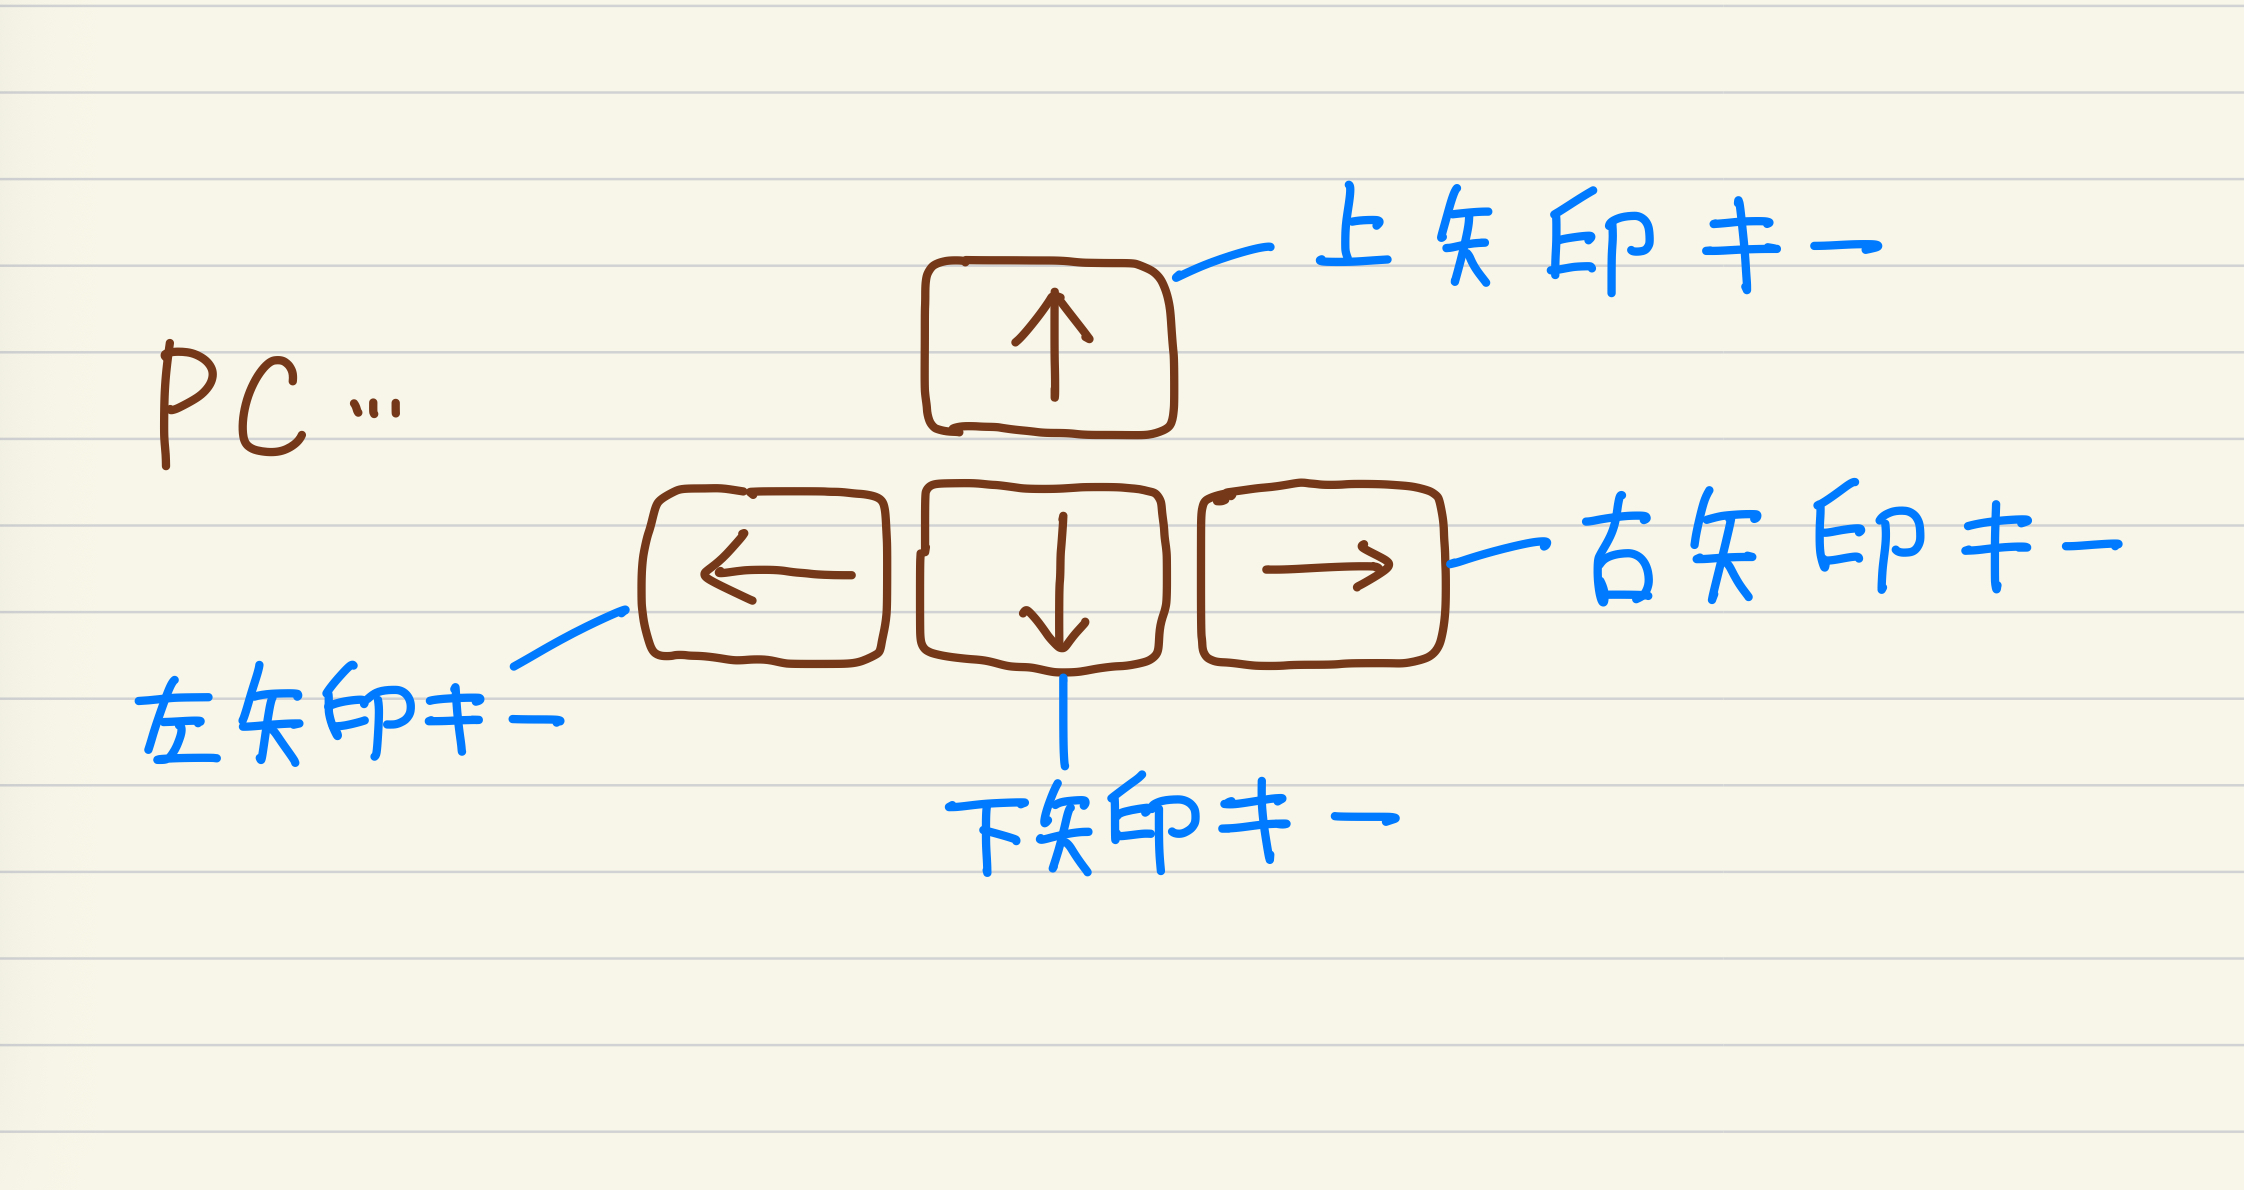
\includegraphics[width=12cm]{imags/PCYajirusiKeyDiscription.eps}
    \caption{PCの矢印キーと名前の対応}
  \end{center}
  \begin{center}
    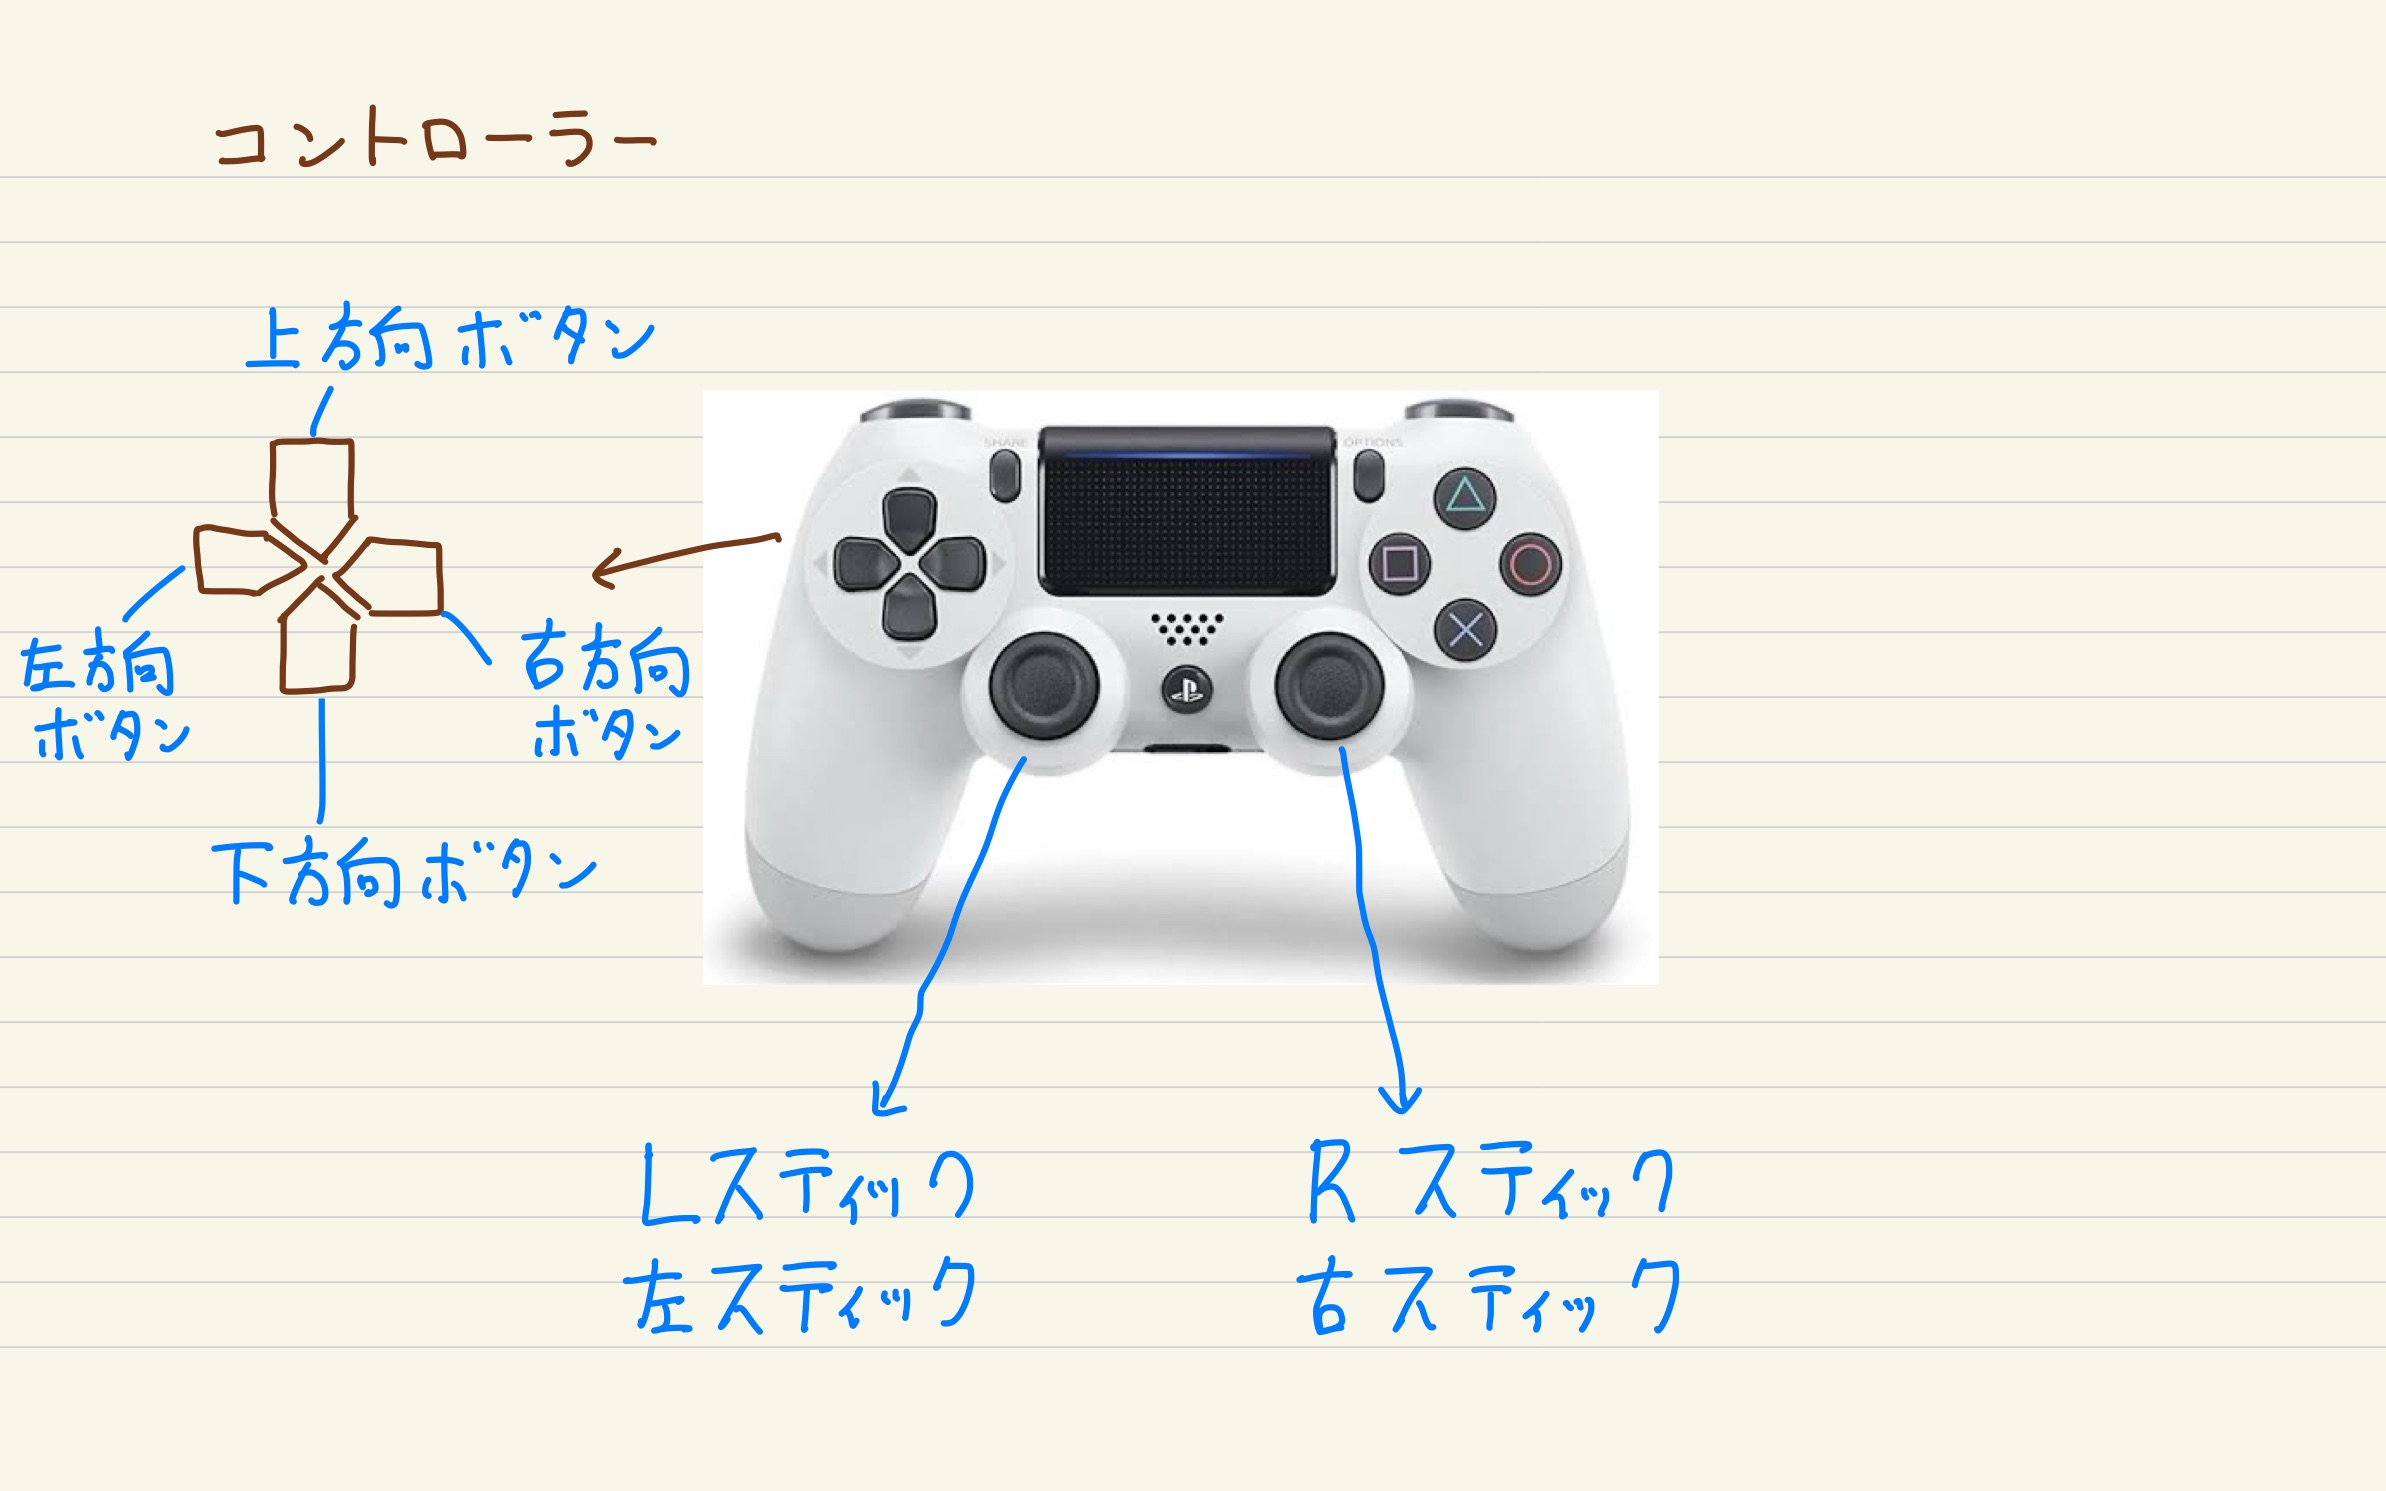
\includegraphics[width=12cm]{imags/ControllerBottunDiscription.eps}
    \caption{コントローラーのボタンと名前の対応}
  \end{center}
\end{figure}

\newpage

・左右移動-要求仕様
\begin{enumerate}
  \item 地面の上で左右に動く
  \item 空中で左右に動く
  \item 左右に動けない時は動かない
  \begin{enumerate}
    \item 移動方向に壁がある時
  \end{enumerate}
\end{enumerate}

\newpage

\subsubsection{ジャンプ}

ジャンプボタンを押すと、大学生が上に飛ぶ。

\begin{figure}[htbp]
  \begin{center}
    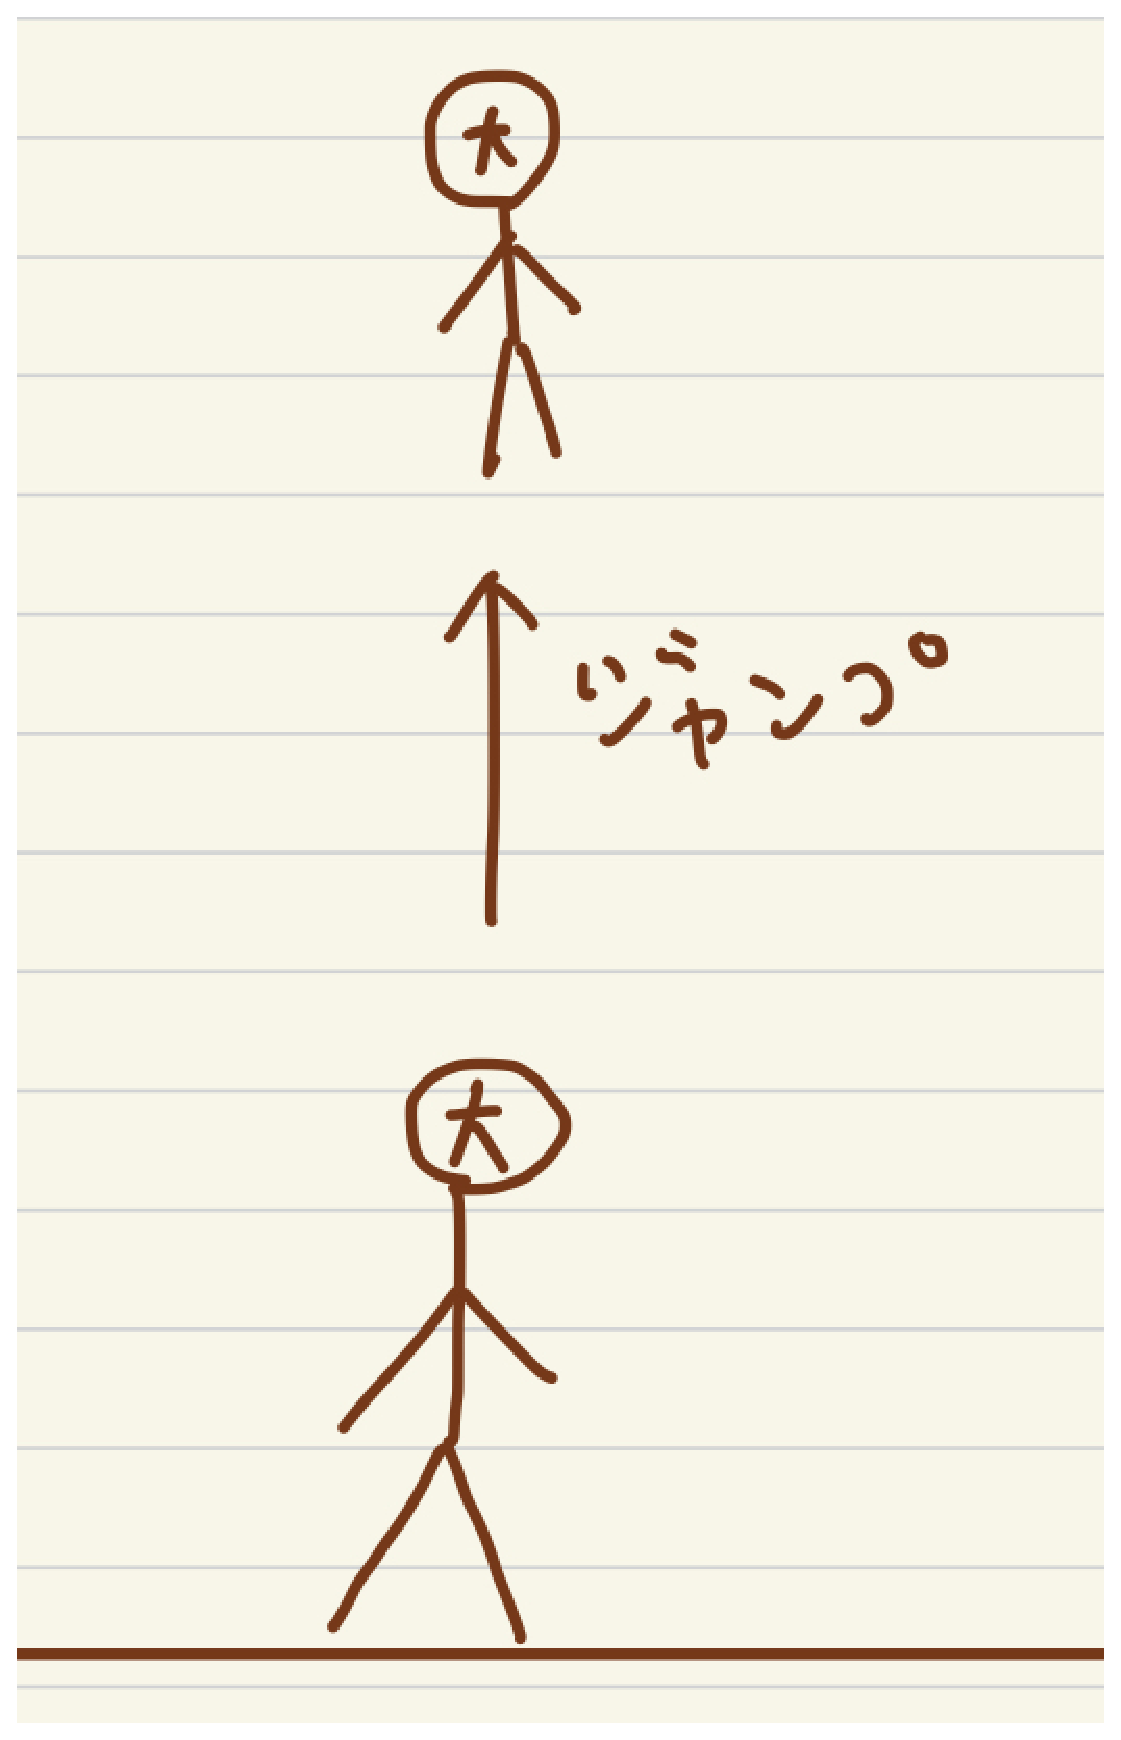
\includegraphics[height=10cm]{imags/jumpDiscription.eps}
    \caption{ジャンプする大学生}
  \end{center}
\end{figure}

\newpage

\begin{table}[htbp]
  \centering
  \caption{ジャンプボタンの対応}
  \begin{tabular}{c|c}
    端末 & キー/ボタン \\
    \hline
    PC & 上矢印キー \\
      & Wキー \\
      & Jキー \\
    \hline
    コントローラー & Aボタン \\
      & 丸ボタン \\
      & Lスティック上弾き入力 (要検討) \\
  \end{tabular}
\end{table}



\end{document}
